% (C) 2024 Yung-Yu Chen.  All rights reserved.
% chktex-file 3
% chktex-file 8
% chktex-file 10
% chktex-file 13
% chktex-file 17
% chktex-file 24
% chktex-file 25
% chktex-file 36
% chktex-file 37

\documentclass{turgon}

%\usepackage{lmodern}

\usepackage[printwatermark]{xwatermark}
\newwatermark[allpages,color=black!15,angle=55,scale=5,xpos=0,ypos=0]%
{DRAFT}

%\doublespacing
\linespread{1.2}

\title{
%
Fit Four-digit NACA Airfoil with Cubic Bezier Curve
%
}

\author{
%
Jie-Yin Lin and Yung-Yu Chen
%
}

%\date{2008.6.4}

\begin{document}

\maketitle

\tableofcontents

%%%%%%%%%%%%%%%%%%%%%%%%%%%%%%%%%%%%%%%%%%%%%%%%%%%%%%%%%%%%%%%%%%%%%%%%%%
%%
\chapter*{Introduction}
\addcontentsline{toc}{chapter}{Introduction}
%%
%%%%%%%%%%%%%%%%%%%%%%%%%%%%%%%%%%%%%%%%%%%%%%%%%%%%%%%%%%%%%%%%%%%%%%%%%%

This file collects notes to fit NACA airfoil by using cubic Bezier curve so
that we can generate mesh for field to be solved by using the CESE
method\cite{chang_method_1995}.

%%%%%%%%%%%%%%%%%%%%%%%%%%%%%%%%%%%%%%%%%%%%%%%%%%%%%%%%%%%%%%%%%%%%%%%%%%
%%
\chapter{Four-digit NACA Airfoil}
% ref: https://en.wikipedia.org/wiki/NACA_airfoil#Five-digit_series

%%
%%%%%%%%%%%%%%%%%%%%%%%%%%%%%%%%%%%%%%%%%%%%%%%%%%%%%%%%%%%%%%%%%%%%%%%%%%

Terminology used for defining the airfoil:
\begin{enumerate}
    \item
    Chord ($c$)
    \item
    Maximum camber ($m$)
    \item
    Maximum camber location ($p$)
    \item
    Maximum thickness ($h$)
    \item
    Camber line (red dashed line)
    \item
    Leading edge ($x = 0, y = 0$)
    \item
    Trailing edge ($x = c, y = 0$)
\end{enumerate}
\begin{figure}[h]
    \centering
    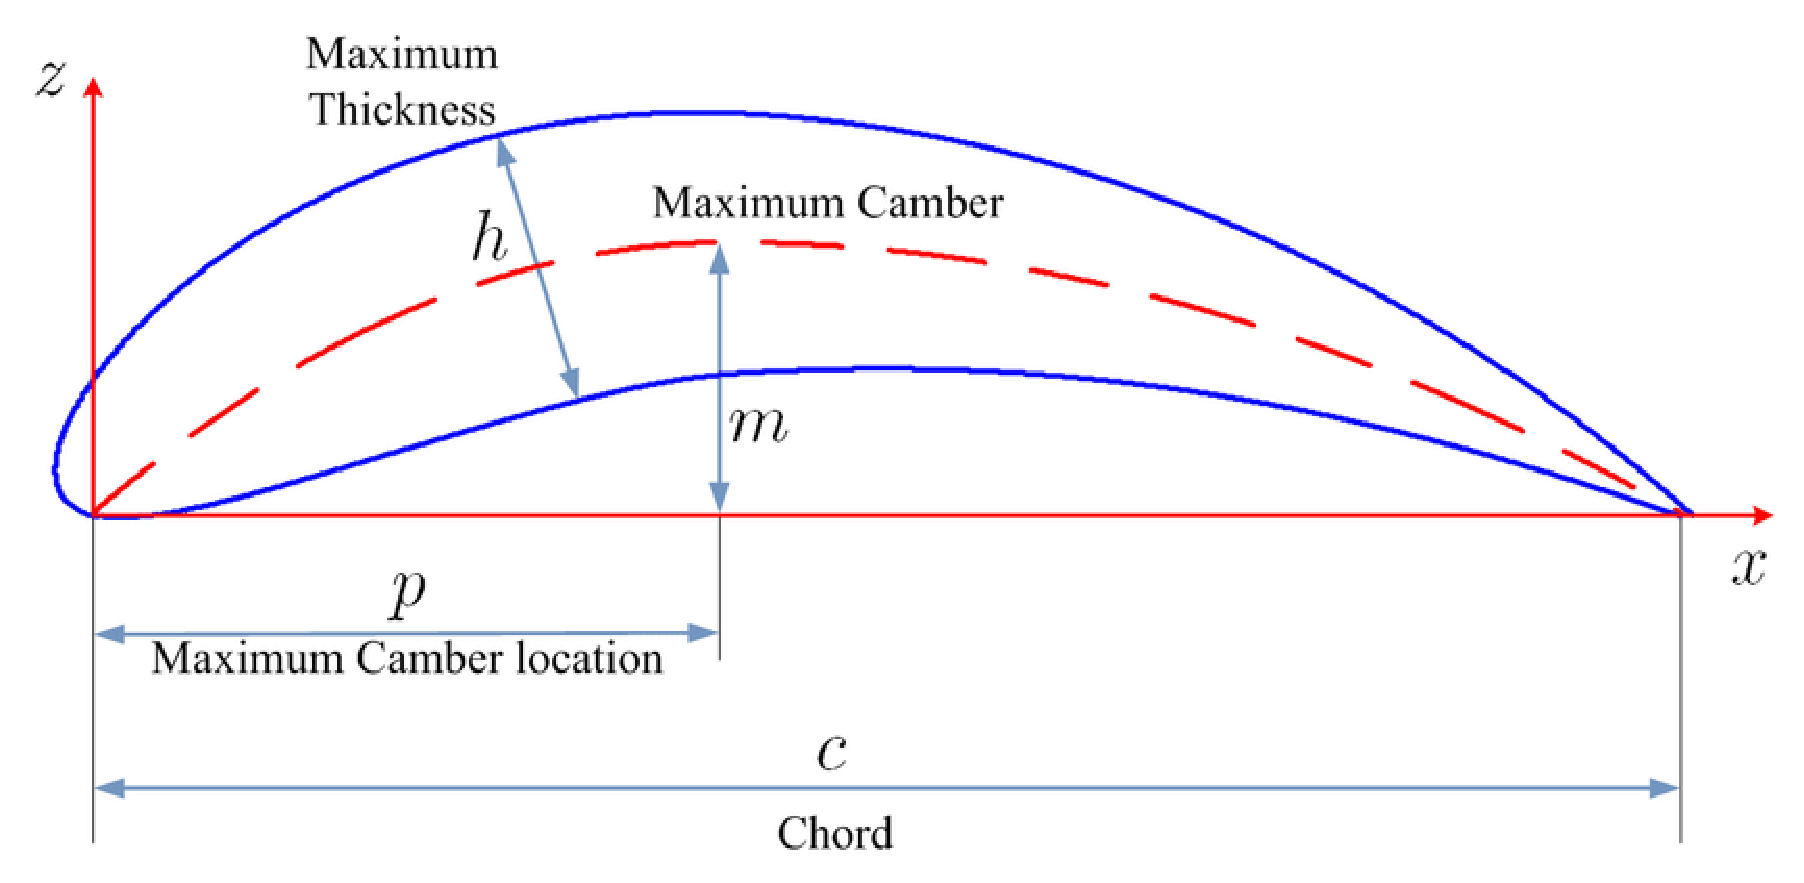
\includegraphics[width=0.5\textwidth]{airfoil_shape_image.eps}
    \caption{The parameters in wing profile.}
    \label{f:airfoil_shape_image}
\end{figure}
% figure downloaded from: https://www.researchgate.net/figure/AIRFOIL-SHAPE-PARAMETERS_fig4_267490031

The wing profile is defined by four-digit ($\mathrm{XYZZ}$):
\begin{enumerate}
    \item
    The 1st digit is the maximum camber as percentage of the chord.
    \begin{equation*}
        m = c \times (\mathrm{X}/100)
    \end{equation*}
    \item
    The 2nd digit is the maximum camber location in tenths of the chord.
    \begin{equation*}
        p = c \times (\mathrm{Y}/10)
    \end{equation*}
    \item
    The last two digits are the maximum thickness as percent of the chord.
    \begin{equation*}
        h = c \times (\mathrm{ZZ}/100)
    \end{equation*}
\end{enumerate}

The formula to calculate the thickness is
\begin{equation*}
    y_h = 5h\left(0.2969\sqrt{x}-0.1260x-0.3516x^2+0.2843x^3-0.1015x^4\right)
\end{equation*}
where $x$ is the position along the chord (from $0$ to $1$), $y_h$ is the
half thickness at a given value of $x$, and $h$ is the maximum thickness.

The camber line equation is
\begin{equation*}
    y_c =
    \begin{cases}
    \frac{m}{p^2} (2px - x^2); & 0 \leq x \leq p \\
    \frac{m}{(1-p)^2} (1 - 2p + 2px - x^2);  &  p \leq x \leq 1
    \end{cases}
\end{equation*}
where $y_c$ is the camber line point at a given value of $x$, $m$ is the
maximum camber, and $p$ is the location of maximum camber.

The point $F_u(x_u, y_u)$ in upper surface equation is
\begin{align}
    x_u &= x - y_h \sin\theta
    \label{e:naca:up_x}
    \\
    y_u &= y_c + y_h \cos\theta
    \label{e:naca:up_y}
\end{align}
and the point $F_l(x_l, y_l)$ in lower surface equation is
\begin{align*}
    x_l &= x + y_h \sin\theta
    \\
    y_l &= y_c - y_h \cos\theta
\end{align*}
where
\begin{equation*}
    \arctan \theta =
    \begin{cases}
    \frac{2m}{p^2} (p - x); & 0 \leq x \leq p \\
    \frac{2m}{(1-p)^2} (p - x);  &  p \leq x \leq 1
    \end{cases}
\end{equation*}

%%%%%%%%%%%%%%%%%%%%%%%%%%%%%%%%%%%%%%%%%%%%%%%%%%%%%%%%%%%%%%%%%%%%%%%%%%
%%
\chapter{Cubic Bezier Curve}
% ref: https://en.wikipedia.org/wiki/B%C3%A9zier_curve#Cubic_B%C3%A9zier_curves

%%
%%%%%%%%%%%%%%%%%%%%%%%%%%%%%%%%%%%%%%%%%%%%%%%%%%%%%%%%%%%%%%%%%%%%%%%%%%

The cubic Bezier curve is defined by 4 controll points $P_0(X_0, Y_0)$,
$P_1(X_1, Y_1)$, $P_2(X_2, Y_2)$, and $P_3(X_3, Y_3)$.
\begin{figure}[h]
    \centering
    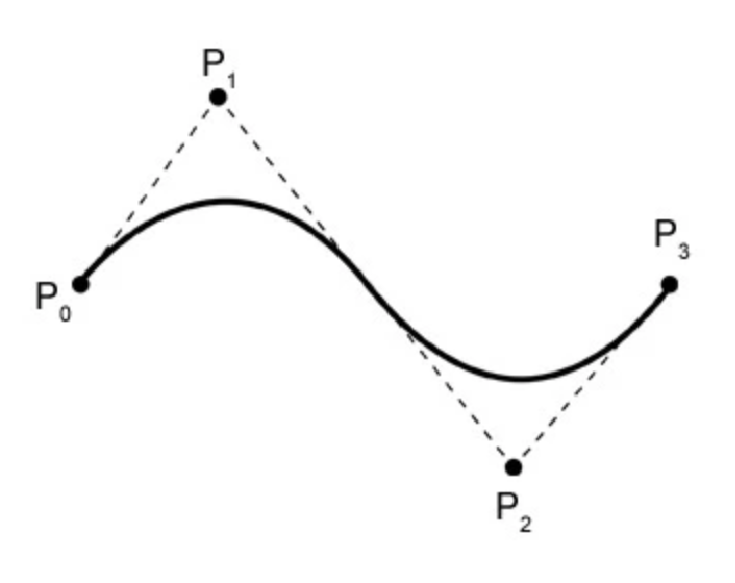
\includegraphics[width=0.3\textwidth]{cubic_bezier_curve.eps}
    \caption{The cubic Bezier curve.}
    \label{f:cubic_bezier_curve}
\end{figure}
% figure downloaded from: https://btnseniorproject17.wordpress.com/2017/05/01/more-unity-part-2-path-following-and-bezier-curves/

The function $B(t)$ is
\begin{equation}
    B(t) = (1-t)^3 P_0 + 3(1-t)^2 t P_1 + 3(1-t) t^2 P_2 + t^3 P_3
    \label{e:cbc:der0}
\end{equation}
where $0 \leq t \leq 1$.  The first-order derivative of $B(t)$ is
\begin{equation}
    B'(t) = 3\left[
      (1-t)^2 (P_1 - P_0) + 2(1-t)t(P_2 - P_1) + t^2(P_3 - P_2)
    \right]
\end{equation}
The second-order derivative of $B(t)$ is
\begin{equation}
    B''(t) = 6\left[(1-t)(P_2 - 2P_1 + P_0) + t(P_3 - 2P_2 + P_1)\right]
\end{equation}
For a sequence of $n+1$ cubic Bezier curves, $B_0(t)$ through $B_n(t)$,
there are $4(n+1)$ controll points can be adjusted. It implies that there
are $4(n+1)$ dimensions of freedom. Assume the first and last points are
fixed. If we wish the value, slope, and curvature between any two Bezier
curves are continuous, the degree of freedom will become $n+2$. Thus, we
can keep the continuous value of curvature when adding the number of Bezier
curves.

%%%%%%%%%%%%%%%%%%%%%%%%%%%%%%%%%%%%%%%%%%%%%%%%%%%%%%%%%%%%%%%%%%%%%%%%%%
%%
\chapter{Linear Least Squares}
% ref: https://en.wikipedia.org/wiki/Linear_least_squares

%%
%%%%%%%%%%%%%%%%%%%%%%%%%%%%%%%%%%%%%%%%%%%%%%%%%%%%%%%%%%%%%%%%%%%%%%%%%%

Linear least squares (LLS) is a set of formulations for solving statistical
problems involved in linear regression, including variants for ordinary,
weighted, and generalized residuals.

Consider the linear equation
\begin{equation}
    Ax = b
    \label{e:lls:leq}
\end{equation}
where $A \in \mathbb{R}^{m \times n}$ and $b \in \mathbb{R}^m$. When $m>n$,
$x \in \mathbb{R}^n$ is the solution of
\begin{equation*}
    \underset{x \in \mathbb{R}^n}{\text{minimize}} ||A x - b||^2
\end{equation*}
$x$ can be computed by
\begin{equation*}
    A^\top A x^* = A^\top b
\end{equation*}
\begin{equation*}
    x^* = (A^\top A)^{-1} A^\top b
    \label{e:lls:sol}
\end{equation*}
where $A^\top$ denotes the transpose of $A$ and $Ax^*$ is the projection of
$b$ in columnn space of $A$.

%%%%%%%%%%%%%%%%%%%%%%%%%%%%%%%%%%%%%%%%%%%%%%%%%%%%%%%%%%%%%%%%%%%%%%%%%%
%%
\chapter{Fit Symmetry Four-digit NACA Airfoil with Cubic Bezier Curve}

%%
%%%%%%%%%%%%%%%%%%%%%%%%%%%%%%%%%%%%%%%%%%%%%%%%%%%%%%%%%%%%%%%%%%%%%%%%%%

We adapt $N$ data points in airfoil upper surface to get the fitting curve.
Compare point $B(t_n)$ in Eq.~(\ref{e:cbc:der0}) with point $F_u(x_i)$ in
Eq.~(\ref{e:naca:up_x_sym}). Here, we fix controll points $P_0$ and $P_3$ at
leading edge and trailing edge. The linear least square equation can be
written as
\begin{equation*}
    \begin{bmatrix}
        3(1 - t_0)^2 t_0 & 3(1 - t_0) t_0^2 \\
        3(1 - t_1)^2 t_1 & 3(1 - t_1) t_1^2 \\
        \vdots & \vdots \\
        3(1 - t_{N-1})^2 t_{N-1} & 3(1 - t_{N-1}) t_{N-1}^2 \\
    \end{bmatrix}
    \begin{bmatrix}
        P_1 \\
        P_2
    \end{bmatrix}
    =
    \begin{bmatrix}
        F_u(x_0) \\
        F_u(x_1) \\
        \vdots \\
        F_u(x_{N-1})
    \end{bmatrix}
    -
    \begin{bmatrix}
        t_0^3 \\
        t_1^3 \\
        \vdots \\
        t_{N-1}^3
    \end{bmatrix}
    P_0 -
    \begin{bmatrix}
        (1 - t_0)^3 \\
        (1 - t_1)^3 \\
        \vdots \\
        (1 - t_{N-1})^3
    \end{bmatrix}
    P_3
\end{equation*}
where
\begin{align*}
    P_0 = 
    \begin{bmatrix}
        0 & 0
    \end{bmatrix}
    \\
    P_3 = 
    \begin{bmatrix}
        c & 0
    \end{bmatrix}
\end{align*}
Then, the controll points $P_1(X_1, Y_1)$ and $P_2(X_2, Y_2)$ can be solved
by Eq.~(\ref{e:lls:sol}).

By adapting a symmetry four-digit NACA airfoil ($\mathrm{00ZZ}$), the
maximum camber ($m$) and maximum camber location ($p$) are equal to $0$.
Then, Eq.~(\ref{e:naca:up_x}) and Eq.~(\ref{e:naca:up_y}) of airfoil upper
surface can be simplified as
\begin{equation}
    x_u = x
    \label{e:naca:up_x_sym}
\end{equation}
\begin{equation}
    y_u = 5h[0.2969\sqrt{x}-0.1260x-0.3516x^2+0.2843x^3-0.1015x^4]
    \label{e:naca:up_y_sym}
\end{equation}

%%%%%%%%%%%%%%%%%%%%%%%%%%%%%%%%%%%%%%%%%%%%%%%%%%%%%%%%%%%%%%%%%%%%%%%%%%
%%
\clearpage
\addcontentsline{toc}{chapter}{Bibliography}
%%
%%%%%%%%%%%%%%%%%%%%%%%%%%%%%%%%%%%%%%%%%%%%%%%%%%%%%%%%%%%%%%%%%%%%%%%%%%

%\bibliographystyle{myunsrtnat} % no sort (order in appearance)
\bibliographystyle{myplainnat} % sort by author
\bibliography{turgon_main}

\end{document}

% vim: set ff=unix fenc=utf8 et sw=2 ts=2 sts=2 tw=79:
